\newcommand{\defs}{../defs}
\documentclass[12pt,oneside,chapterprefix=true]{scrbook}

\usepackage[T1]{fontenc}
\usepackage[utf8x]{inputenc}
\usepackage[brazilian]{babel}
\usepackage[table]{xcolor}
\usepackage{minted}
\usepackage[a5paper,left=0.7cm,right=0.7cm,top=2cm,bottom=2.5cm,]{geometry}
\usepackage{url}
\usepackage{graphicx}
\usepackage[export]{adjustbox}
\usepackage{hyperref}
\usepackage[square]{natbib}
\usepackage[parfill]{parskip}
\usepackage{mdframed}
\usepackage{longtable}
\usepackage{soul}
\usepackage{tabularx}
\usepackage[shortlabels]{enumitem}
\usepackage{xifthen}
\usepackage{multirow}
\usepackage[portuguese, ruled, vlined, linesnumbered, algochapter]{algorithm2e}
\usepackage{amsmath}
\usepackage{amssymb}
\usepackage{amsthm}
\usepackage{tablefootnote}
\usepackage{subfigure}
\usepackage{gensymb}
\usepackage{pgfplots}
\usepackage{xpatch}
\usepackage{varwidth}
\usepackage[htt]{hyphenat}

\renewcommand{\familydefault}{\sfdefault}

\newcommand{\name}{Prof. Marcelo de Souza}
\newcommand{\email}{marcelo.desouza@udesc.br}
\newcommand{\course}{Bacharelado em Engenharia de Software}
\newcommand{\university}{Universidade do Estado de Santa Catarina}
\newcommand{\campus}{Centro de Educação Superior do Alto Vale do Itajaí}
\newcommand{\shortuniversity}{UDESC Ibirama}
\newcommand{\version}{Versão compilada em \today}
\newcommand{\exercisedescription}{Exercício}

\usepackage[automark,headsepline,footsepline]{scrlayer-scrpage}
\lehead{\content}
\lohead{\content}
\rehead{}
\rohead{}
\cehead{}
\cohead{}
\lefoot{\name}
\lofoot{\name}
\refoot{\\\thepage}
\rofoot{\\\thepage}
\cofoot{}
\cefoot{}
\setkomafont{pagehead}{\normalfont\small}
\setkomafont{pagefoot}{\normalfont}

\newpairofpagestyles{firstpage}{}

\newcommand{\makeheader}{
	\thispagestyle{firstpage}
	\vspace*{-42pt}
	\framebox[\textwidth]{
		\parbox{0.97\textwidth}{
			\begin{center}
				{\scriptsize\shortcourse\ -- \class}
				
				\vspace{10pt}
				
				\textbf{\content}
				
				\vspace{2pt}
				
				{\small\name}
				
				\vspace{10pt}
				
				{\scriptsize\shortuniversity\hfill\email}
				
				\vspace{-5pt}
				
				{\scriptsize\course\hfill\version}
				
			\end{center}
		}
	}
%	\vspace{-15pt}
%	\begin{flushright}
%		{\scriptsize\source}
%	\end{flushright}
	\smallskip
}

\renewcommand{\thesection}{\arabic{section}}

\allowdisplaybreaks

\hypersetup{
	colorlinks,
	linkcolor={blue!80!black},
	citecolor={blue!80!black},
	urlcolor={blue!80!black}
}

\definecolor{codelinecolor}{gray}{.90}
\colorlet{codeboxcolor}{blue!8}

\surroundwithmdframed{minted}

\BeforeBeginEnvironment{mdframed}{}
\AfterEndEnvironment{mdframed}{}

\mdfsetup{%
	backgroundcolor=codeboxcolor,
	linecolor=white}

\setminted{%
	mathescape,
	escapeinside=@@,
	linenos,
	breaklines,
	tabsize=3,
	fontsize=\footnotesize}

\newcommand{\code}[1]{%
	\sethlcolor{codelinecolor}
	\texttt{\hl{#1}}%
}

\newcommand{\inblock}[1]{%
	\sethlcolor{blockcolor}
	\hl{\mbox{#1}}%
}

\newcommand{\javacode}[1]{%
	\mintinline[escapeinside=~~]{java}{#1}
}

\newcommand{\javacodecolor}[1]{%
	\mintinline[escapeinside=~~,bgcolor=codeboxcolor]{java}{#1}
}

\newcounter{number}
\newenvironment{exercise}[1][]
{%
	\refstepcounter{number}%
	\noindent%
	\ifthenelse{\equal{#1}{}}%
		{\textbf{\exercisedescription~\thenumber.\\}}%
		{\textbf{\exercisedescription~\thenumber. (#1)\\}}%
	\rmfamily%
}{\medskip}%

\newcommand{\resetexercisenumbering}{
	\setcounter{number}{0}
}

\newcounter{solutionnumber}
\newenvironment{solution}[1][]
{%
	\refstepcounter{solutionnumber}%
	\noindent%
	\ifthenelse{\equal{#1}{}}%
	{\textbf{Solução -- \exercisedescription~\thesolutionnumber.\\}}%
	{\textbf{Solução -- \exercisedescription~\thesolutionnumber. (#1)\\}}%
	\rmfamily%
}{\medskip}%

\makeatletter%
\setlength{\@fptop}{5pt}

\def\arraystretch{1.5}

\newcommand{\insertspace}{\vspace{1.2em}}
\newcommand{\removespace}{\vspace{-1.2em}}

\setlength{\fboxsep}{0.8em}

\usepackage{array}
\newcolumntype{L}[1]{>{\raggedright\let\newline\\\arraybackslash\hspace{0pt}}m{#1}}
\newcolumntype{C}[1]{>{\centering\let\newline\\\arraybackslash\hspace{0pt}}m{#1}}
\newcolumntype{R}[1]{>{\raggedleft\let\newline\\\arraybackslash\hspace{0pt}}m{#1}}

\colorlet{blockcolor}{red!25}
\colorlet{redtext}{red!60!black}

\newcommand{\block}[1]{%
	\medskip
	\begin{figure}[H]
		\centering
		\begin{tikzpicture}
		\node [rectangle, align=center, fill=blockcolor, rounded corners=0.04cm, opacity = 1, text opacity = 1] {%
			#1
		};
		\end{tikzpicture}
	\end{figure}
}

\newcommand{\newtitle}[1]{%
	\begin{figure}[H]
		\begin{tikzpicture}
		\node [rectangle, fill=blue!30, rounded corners=0.04cm, opacity=1, text opacity=1, minimum width=\textwidth, text width=\linewidth-2*\pgfkeysvalueof{/pgf/inner xsep}, align=left] {%
			\textbf{#1}
		};
		\end{tikzpicture}
	\end{figure}
	\vspace{-10pt}
}

\renewcommand{\qedsymbol}{$\blacksquare$}
\xpatchcmd{\proof}{\itshape}{\normalfont\bfseries}{}{}

\newcommand{\content}{Introdução}
\newcommand{\class}{Algoritmos e Estruturas de Dados}
\newcommand{\shortcourse}{45EST}

\begin{document}

\makeheader

Leitura obrigatória:
\begin{itemize}
	\item Capítulo 2 de~\cite{EdelweissAndGalante2009} -- Conceitos básicos.
\end{itemize}
Leitura complementar:
\begin{itemize}
	\item Capítulo 1 de~\cite{Pereira2008} -- Introdução.
\end{itemize}

\medskip

\newtitle{Conceitos básicos}

Algumas definições:
\begin{itemize}
	\item \textbf{Algoritmo:} sequência de passos para realizar uma tarefa.
	\item \textbf{Estrutura de dados:} forma sistemática de organizar e acessar os dados.
\end{itemize}

\textbf{Objetivo:} escolher os melhores componentes para resolver um problema.

\medskip

\textbf{Exemplo}

Jogo para coleta de itens em uma grade (figura abaixo):
\begin{itemize}
	\item \textbf{`X'}: item com valor 100.
	\item \textbf{`O'}: item com valor 200.
	\item Representação do cenário: matriz $n \times n$.
	\item Operações:
	\begin{enumerate}
		\item Varrer ambiente.
		\item Encontrar o item mais próximo.
	\end{enumerate}
\end{itemize}

\begin{figure}[H]
	\centering
	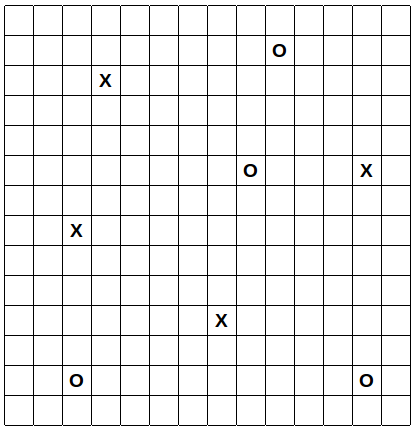
\includegraphics[width=0.6\linewidth]{img/cenario}
\end{figure}

{\color{redtext}
Qual o consumo de memória e tempo de processamento?
\begin{itemize}
	\item Cenário $10 \times 10$.
	\item Cenário $1000 \times 1000$.
	\item Cenário $10000 \times 10000$.
\end{itemize}
}

\block{
	Quanto tempo demora para executar as operações?\\
	Quanta memória é consumida para armazenar o cenário?
}

\textbf{Solução:} usar uma estrutura de dados mais eficiente!

\clearpage

Linguagens de programação fornecem:
\begin{itemize}
	\item Tipos de dados primitivos: inteiro, real, lógico...
	\item Tipos de dados estruturados: arranjos, registros, sequências...
\end{itemize}

\medskip

Usar esses recursos para criar:
\begin{itemize}
	\item TAD (tipo abstrato de dados): estruturas definidas pelo usuário.
	\begin{itemize}
		\item Organização dos dados.
		\item Operações sobre os dados.
	\end{itemize}
\end{itemize}

\medskip

Representação física:
\begin{itemize}
	\item Contiguidade física
	\begin{itemize}
		\item Ex: vetores e matrizes.
		\item Valores armazenados sequencialmente na memória.
		\item $\oplus$ rápido acesso.
		\item $\ominus$ espaço físico estático.
	\end{itemize}
	\item Encadeamento
	\begin{itemize}
		\item Ex: listas, pilhas e filas.
		\item Alocação (não sequencial) dinâmica de memória.
		\item $\oplus$ maleabilidade.
		\item $\ominus$ acesso serial.
	\end{itemize}
\end{itemize}

\clearpage

\newtitle{Atividades}

\begin{enumerate}
	\item Implemente o exemplo do jogo para coleta de itens. Verifique a memória utilizada e o tempo de processamento das operações em função dos diferentes tamanhos da grade. Verifique qual o limite de tamanho capaz de ser processado.
	
	\item Proponha uma nova estrutura de dados, capaz de utilizar menos memória e melhorar o desempenho na execução das operações. Verifique o novo limite de tamanho capaz de ser processado.
\end{enumerate}

\medskip

\newtitle{Referências}
\begingroup
	\footnotesize
	\renewcommand{\chapter}[2]{}%
	\bibliographystyle{apalike}
	\bibliography{../referencias}
\endgroup

\end{document}